\documentclass{standalone}
\usepackage{tikz}
\usetikzlibrary{patterns, positioning}
\usepackage[sfdefault]{ClearSans} %% option 'sfdefault' activates Clear Sans as the default text font
\usepackage[T1]{fontenc}

\begin{document}
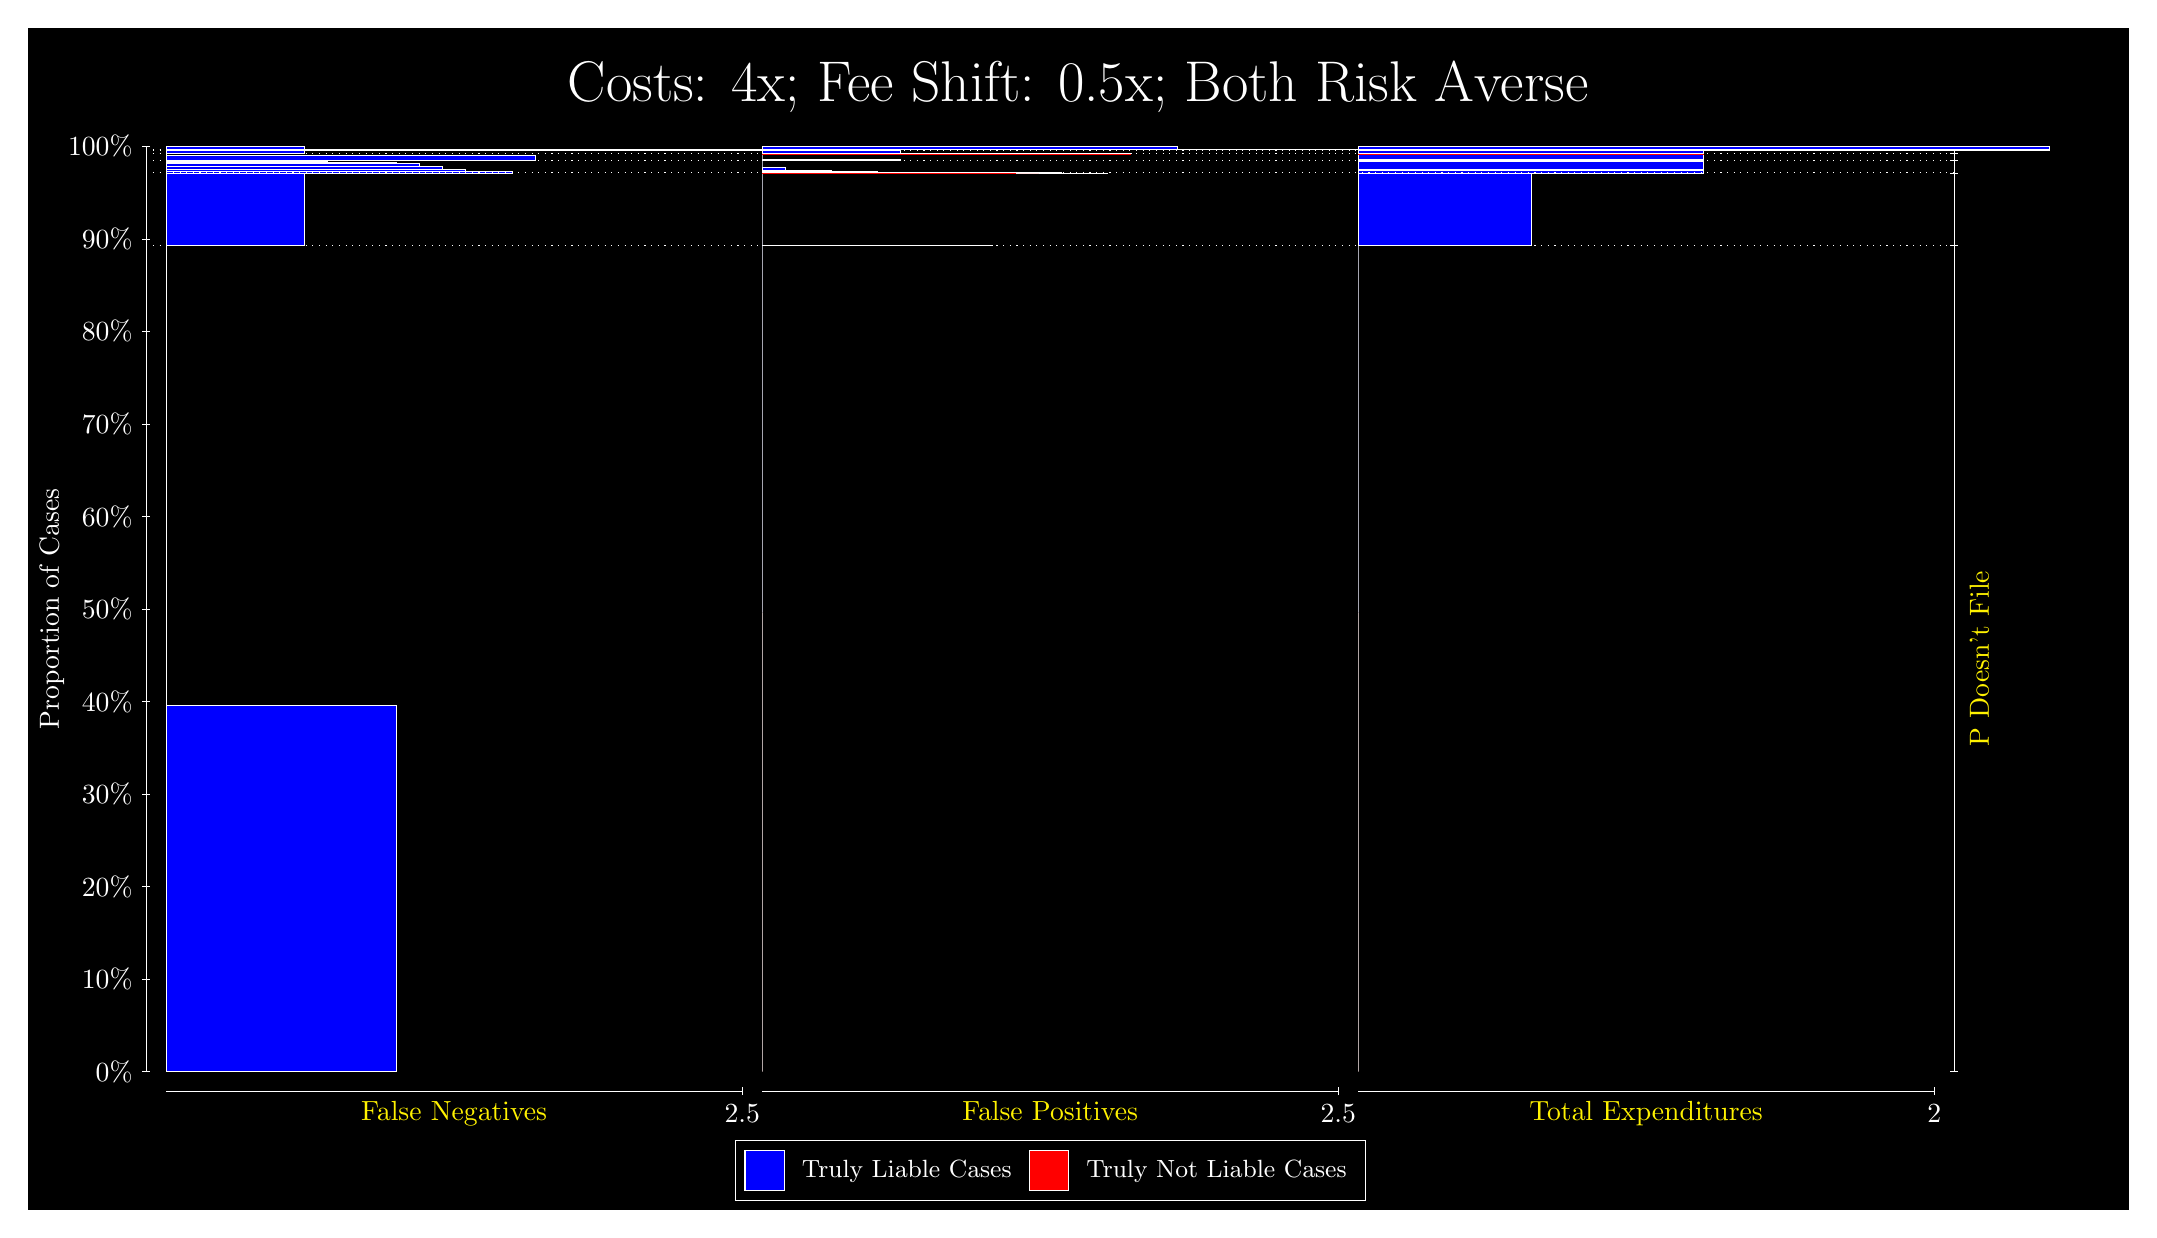
\begin{tikzpicture}
\draw[fill=black] (0,0) rectangle (26.667,15);
\draw[text=white] (0,13.5) rectangle (26.667,15) node[midway] {\huge Costs: 4x; Fee Shift: 0.5x; Both Risk Averse};
\draw[white, very thin] (1.5,1.75) -- (1.5,13.5);
\node[rotate=90, text=white, anchor=center] at (0.3, 7.625) {Proportion of Cases};
\draw[white, very thin] (1.45,1.75) -- (1.55,1.75);
\node[text=white, anchor=east] at (1.45, 1.75) {0\%};
\draw[white, very thin] (1.45,2.925) -- (1.55,2.925);
\node[text=white, anchor=east] at (1.45, 2.925) {10\%};
\draw[white, very thin] (1.45,4.1) -- (1.55,4.1);
\node[text=white, anchor=east] at (1.45, 4.1) {20\%};
\draw[white, very thin] (1.45,5.275) -- (1.55,5.275);
\node[text=white, anchor=east] at (1.45, 5.275) {30\%};
\draw[white, very thin] (1.45,6.45) -- (1.55,6.45);
\node[text=white, anchor=east] at (1.45, 6.45) {40\%};
\draw[white, very thin] (1.45,7.625) -- (1.55,7.625);
\node[text=white, anchor=east] at (1.45, 7.625) {50\%};
\draw[white, very thin] (1.45,8.8) -- (1.55,8.8);
\node[text=white, anchor=east] at (1.45, 8.8) {60\%};
\draw[white, very thin] (1.45,9.975) -- (1.55,9.975);
\node[text=white, anchor=east] at (1.45, 9.975) {70\%};
\draw[white, very thin] (1.45,11.15) -- (1.55,11.15);
\node[text=white, anchor=east] at (1.45, 11.15) {80\%};
\draw[white, very thin] (1.45,12.325) -- (1.55,12.325);
\node[text=white, anchor=east] at (1.45, 12.325) {90\%};
\draw[white, very thin] (1.45,13.5) -- (1.55,13.5);
\node[text=white, anchor=east] at (1.45, 13.5) {100\%};

\draw[white, very thin] (24.457,1.75) -- (24.457,13.5);
\draw[white, very thin] (24.407,1.75) -- (24.507,1.75);
\node[anchor=west] at (24.407, 1.75) {};
\draw[white, very thin] (24.407,12.237) -- (24.507,12.237);
\node[anchor=west] at (24.407, 12.237) {};
\draw[white, very thin] (24.407,13.163) -- (24.507,13.163);
\node[anchor=west] at (24.407, 13.163) {};
\draw[white, very thin] (24.407,13.319) -- (24.507,13.319);
\node[anchor=west] at (24.407, 13.319) {};
\draw[white, very thin] (24.407,13.406) -- (24.507,13.406);
\node[anchor=west] at (24.407, 13.406) {};
\draw[white, very thin] (24.407,13.453) -- (24.507,13.453);
\node[anchor=west] at (24.407, 13.453) {};
\draw[white, very thin] (24.407,13.464) -- (24.507,13.464);
\node[anchor=west] at (24.407, 13.464) {};
\draw[white, very thin] (24.407,13.5) -- (24.507,13.5);
\node[anchor=west] at (24.407, 13.5) {};

\draw[white, very thin, fill=blue] (1.75,1.75) rectangle (4.6775,6.4064);
\draw[white, very thin, fill=red] (1.75,6.4064) rectangle (1.75,12.237);
\draw[white, very thin, fill=blue] (1.75,12.237) rectangle (3.5065,13.155);
\draw[white, very thin, fill=red] (1.75,13.155) rectangle (1.75,13.163);
\draw[white, very thin, fill=blue] (1.75,13.163) rectangle (6.1413,13.181);
\draw[white, very thin, fill=blue] (1.75,13.181) rectangle (5.8486,13.186);
\draw[white, very thin, fill=blue] (1.75,13.186) rectangle (5.5558,13.214);
\draw[white, very thin, fill=blue] (1.75,13.214) rectangle (5.2631,13.252);
\draw[white, very thin, fill=blue] (1.75,13.252) rectangle (4.9703,13.282);
\draw[white, very thin, fill=blue] (1.75,13.282) rectangle (4.6775,13.292);
\draw[white, very thin, fill=blue] (1.75,13.292) rectangle (4.3848,13.299);
\draw[white, very thin, fill=blue] (1.75,13.299) rectangle (4.092,13.303);
\draw[white, very thin, fill=blue] (1.75,13.303) rectangle (3.7993,13.307);
\draw[white, very thin, fill=red] (1.75,13.307) rectangle (1.75,13.319);
\draw[white, very thin, fill=blue] (1.75,13.319) rectangle (6.4341,13.392);
\draw[white, very thin, fill=red] (1.75,13.392) rectangle (1.75,13.406);
\draw[white, very thin, fill=blue] (1.75,13.406) rectangle (3.5065,13.452);
\draw[white, very thin, fill=red] (1.75,13.452) rectangle (1.75,13.453);
\draw[white, very thin, fill=blue] (1.75,13.453) rectangle (9.9471,13.457);
\draw[white, very thin, fill=red] (1.75,13.457) rectangle (1.75,13.464);
\draw[white, very thin, fill=blue] (1.75,13.464) rectangle (3.5065,13.498);
\draw[white, very thin, fill=red] (1.75,13.498) rectangle (1.75,13.5);
\draw[white, very thin, fill=red] (9.3189,1.75) rectangle (9.3189,7.581);
\draw[white, very thin, fill=blue] (9.3189,7.581) rectangle (9.3189,12.237);
\draw[white, very thin, fill=red] (9.3189,12.237) rectangle (12.246,12.246);
\draw[white, very thin, fill=blue] (9.3189,12.246) rectangle (9.3189,13.163);
\draw[white, very thin, fill=red] (9.3189,13.163) rectangle (13.71,13.164);
\draw[white, very thin, fill=red] (9.3189,13.164) rectangle (13.417,13.164);
\draw[white, very thin, fill=red] (9.3189,13.164) rectangle (13.125,13.165);
\draw[white, very thin, fill=red] (9.3189,13.165) rectangle (12.832,13.165);
\draw[white, very thin, fill=red] (9.3189,13.165) rectangle (12.539,13.167);
\draw[white, very thin, fill=red] (9.3189,13.167) rectangle (12.246,13.168);
\draw[white, very thin, fill=red] (9.3189,13.168) rectangle (11.954,13.17);
\draw[white, very thin, fill=red] (9.3189,13.17) rectangle (11.661,13.171);
\draw[white, very thin, fill=red] (9.3189,13.171) rectangle (11.368,13.175);
\draw[white, very thin, fill=blue] (9.3189,13.175) rectangle (10.783,13.179);
\draw[white, very thin, fill=blue] (9.3189,13.179) rectangle (10.49,13.183);
\draw[white, very thin, fill=blue] (9.3189,13.183) rectangle (10.197,13.19);
\draw[white, very thin, fill=blue] (9.3189,13.19) rectangle (9.9044,13.201);
\draw[white, very thin, fill=blue] (9.3189,13.201) rectangle (9.6116,13.231);
\draw[white, very thin, fill=blue] (9.3189,13.231) rectangle (9.3189,13.319);
\draw[white, very thin, fill=red] (9.3189,13.319) rectangle (11.075,13.333);
\draw[white, very thin, fill=blue] (9.3189,13.333) rectangle (9.3189,13.406);
\draw[white, very thin, fill=red] (9.3189,13.406) rectangle (14.003,13.408);
\draw[white, very thin, fill=blue] (9.3189,13.408) rectangle (11.075,13.453);
\draw[white, very thin, fill=red] (9.3189,13.453) rectangle (11.075,13.46);
\draw[white, very thin, fill=blue] (9.3189,13.46) rectangle (9.3189,13.464);
\draw[white, very thin, fill=red] (9.3189,13.464) rectangle (17.516,13.465);
\draw[white, very thin, fill=blue] (9.3189,13.465) rectangle (14.588,13.5);
\draw[white, very thin, fill=red] (16.888,1.75) rectangle (16.888,7.581);
\draw[white, very thin, fill=blue] (16.888,7.581) rectangle (16.888,12.237);
\draw[white, very thin, fill=red] (16.888,12.237) rectangle (19.083,12.246);
\draw[white, very thin, fill=blue] (16.888,12.246) rectangle (19.083,13.163);
\draw[white, very thin, fill=red] (16.888,13.163) rectangle (21.279,13.164);
\draw[white, very thin, fill=blue] (16.888,13.164) rectangle (21.279,13.195);
\draw[white, very thin, fill=red] (16.888,13.195) rectangle (21.279,13.204);
\draw[white, very thin, fill=blue] (16.888,13.204) rectangle (21.279,13.307);
\draw[white, very thin, fill=red] (16.888,13.307) rectangle (21.279,13.308);
\draw[white, very thin, fill=blue] (16.888,13.308) rectangle (21.279,13.319);
\draw[white, very thin, fill=red] (16.888,13.319) rectangle (21.279,13.333);
\draw[white, very thin, fill=blue] (16.888,13.333) rectangle (21.279,13.406);
\draw[white, very thin, fill=red] (16.888,13.406) rectangle (21.279,13.408);
\draw[white, very thin, fill=blue] (16.888,13.408) rectangle (21.279,13.453);
\draw[white, very thin, fill=red] (16.888,13.453) rectangle (25.67,13.46);
\draw[white, very thin, fill=blue] (16.888,13.46) rectangle (25.67,13.464);
\draw[white, very thin, fill=red] (16.888,13.464) rectangle (25.67,13.465);
\draw[white, very thin, fill=blue] (16.888,13.465) rectangle (25.67,13.5);
\draw[white, dotted] (1.5,12.237) -- (24.457,12.237);
\draw[white, dotted] (1.5,13.163) -- (24.457,13.163);
\draw[white, dotted] (1.5,13.319) -- (24.457,13.319);
\draw[white, dotted] (1.5,13.406) -- (24.457,13.406);
\draw[white, dotted] (1.5,13.453) -- (24.457,13.453);
\draw[white, dotted] (1.5,13.464) -- (24.457,13.464);
\draw[white, very thin] (1.75,1.5) -- (9.0689,1.5);
\node[text=yellow, anchor=north] at (5.4094, 1.5) {False Negatives};
\draw[white, very thin] (9.0689,1.45) -- (9.0689,1.55);
\node[text=white, anchor=north] at (9.0689, 1.45) {2.5};

\draw[white, very thin] (9.3189,1.5) -- (16.638,1.5);
\node[text=yellow, anchor=north] at (12.978, 1.5) {False Positives};
\draw[white, very thin] (16.638,1.45) -- (16.638,1.55);
\node[text=white, anchor=north] at (16.638, 1.45) {2.5};

\draw[white, very thin] (16.888,1.5) -- (24.207,1.5);
\node[text=yellow, anchor=north] at (20.547, 1.5) {Total Expenditures};
\draw[white, very thin] (24.207,1.45) -- (24.207,1.55);
\node[text=white, anchor=north] at (24.207, 1.45) {2};

\node[text=yellow, centered, rotate=90] at (24.777, 6.9937) {P Doesn't File};







\draw (12.978300999999998,1.5) node[draw=none] (baseCoordinate) {};
\begin{scope}[align=center]
        \matrix[scale=0.5, draw=white, below=0.5cm of baseCoordinate, nodes={draw}, column sep=0.1cm]{
            \node[rectangle, draw, minimum width=0.5cm, minimum height=0.5cm, fill=blue] {}; &
            \node[draw=none, font=\small, text=white] (B) {Truly Liable Cases}; &
            \node[rectangle, draw, minimum width=0.5cm, minimum height=0.5cm, fill=red] {}; &
            \node[draw=none, font=\small, text=white] (B) {Truly Not Liable Cases}; \\
            };
\end{scope}

\end{tikzpicture}
\end{document}